\section{问题四：最终模型与验证结果}

\subsection{非线性残差模型的路线比较}

前三问得到两个基本结论：一方面，固定多声道积分能够给出稳定且具有明确物理意义的流量主尺度；另一方面，D0 正常工况曲线虽可修正流量相关系统偏差，却不能完整补偿弯管、旋流等因素引起的附加剖面畸变。因此，问题四的重点是在物理基线上逐步提高残差模型的表达能力与稳定性。依据超声流量计的数据驱动修正、物理约束和小样本正则化理论\cite{Zhao2014ANN,Li2023MLInUse,Cai2025PhysConstrainedGAN,Scholkopf2002LearningKernels}，本文依次建立 Ridge、ANN、紧凑 RBF-KRR、物理--稳定性双核 KRR 和受约束 D0-RBF 后校准双核 KRR：Ridge 用于检验紧凑剖面特征是否有效，ANN 用于检验非线性补偿是否必要，紧凑 RBF-KRR 用于在小样本下实现受控非线性，双核 KRR 进一步描述逐秒稳定性，后校准模型则用于平衡给定标定窗口上的综合指标。模型关系如图~\ref{fig:problem4_engineering_pipeline} 所示。高维全量拟合仅用于估计样本内表达上界，不参与泛化模型的选择。

\begin{figure}[H]
  \centering
  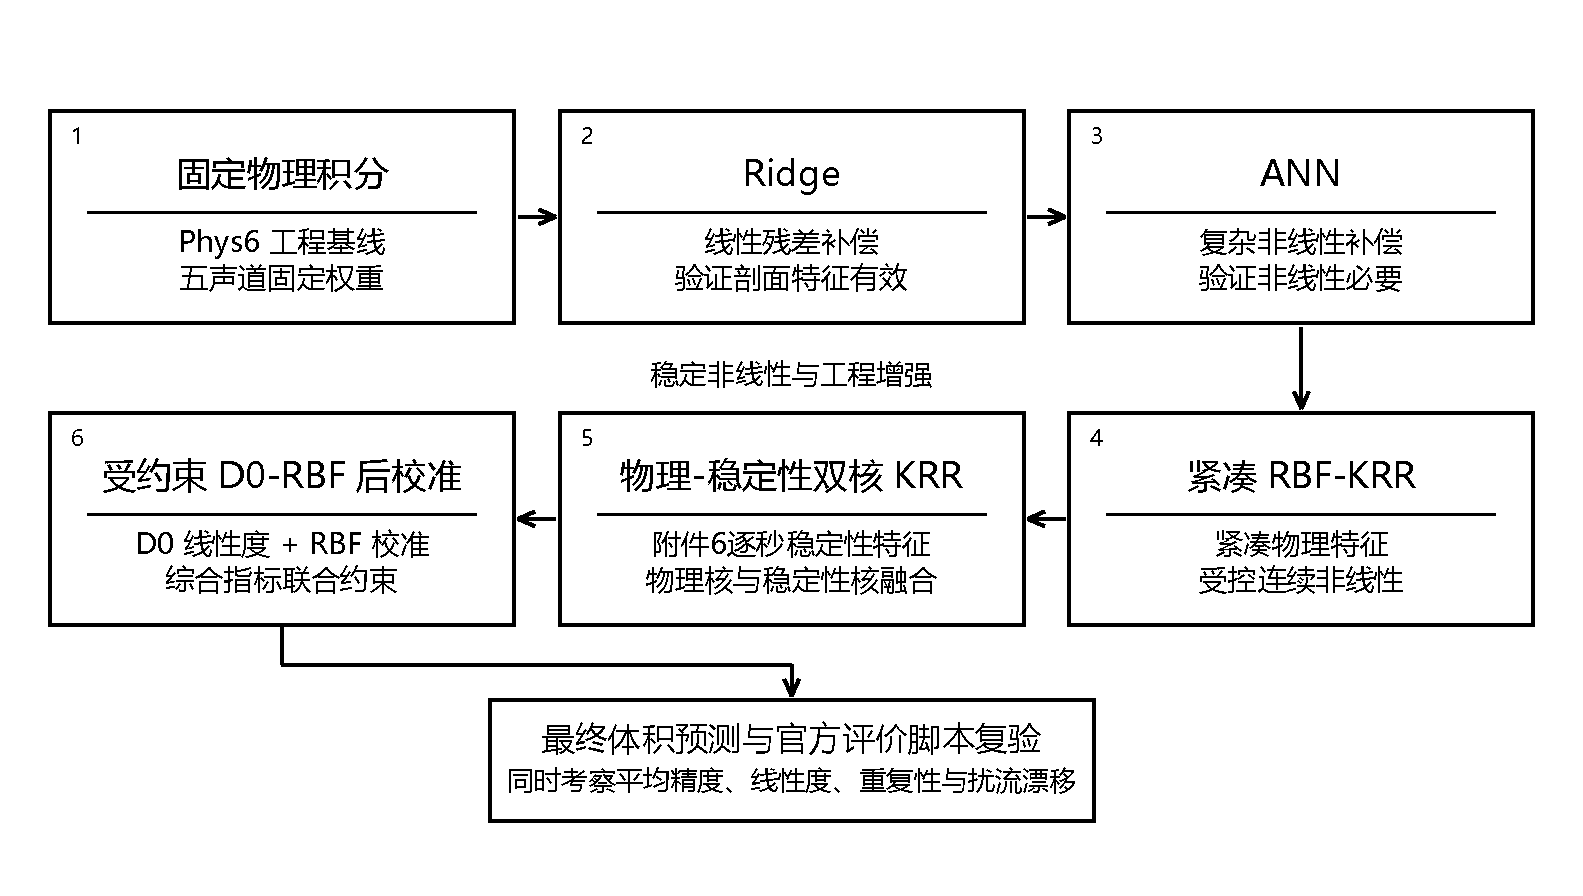
\includegraphics[width=0.98\textwidth]{../figures/fig_problem4_engineering_pipeline.pdf}
  \caption{问题四模型递进的工程方框图}
  \label{fig:problem4_engineering_pipeline}
\end{figure}

除全量拟合基准外，Ridge、ANN 与 KRR 均采用相同的标签盲划分，其中 $118$ 个窗口构成训练集，$41$ 个窗口构成验证集。划分过程按 $h=(\mathrm{date},\mathrm{flow\ point},\mathrm{disturbance\ id})$ 保持重复单元覆盖；日期、窗口编号和人工扰流编号不作为模型输入，特征标准化参数、D0 校准曲线及模型系数均由训练集估计。评价指标包括窗口 MAE、按 $g=(\mathrm{date},\mathrm{flow\ point})$ 构成的评价组、$\max_g|\bar e_g|$ 以及 $u_{\mathrm{nor},L}$、$u_{\mathrm{nor},r}$、$u_{\mathrm{nor},d}$。

\noindent{\circlednumberfont ①}全量拟合基准\par

为检验现有运行时变量对标签的最大表达能力，本文以 Lagrange 体积为基线，将流量尺度、声道、剖面、动态、零点及其平方项和部分交互项扩展为 $358$ 个多项式特征，用带极小正则项的线性模型学习相对修正：
\begin{equation}
\begin{aligned}
r_i
&=\frac{V_i^{\mathrm{std}}}{V_{\mathrm{Lag},i}}-1,\\
\hat V_i
&=V_{\mathrm{Lag},i}
\left(1+\boldsymbol\beta^{\mathsf T}\boldsymbol\phi_i\right).
\end{aligned}
\end{equation}
其中 $\boldsymbol\phi_i$ 为多项式特征，正则化参数为 $\lambda=10^{-9}$。问题一中 Phys6 与 Lagrange 的总体 MAE 分别为 $0.180653\%$ 和 $0.183613\%$，而两者的平均误差分别为 $-0.136424\%$ 和 $-0.007930\%$。为估计高维残差映射的样本内表达上限，本节采用平均偏差较小的 Lagrange 作为近插值基线；泛化模型仍采用总体 MAE 较低的 Phys6。该模型使用全部 $159$ 个窗口的标签进行估计，但运行时输入不含日期、窗口编号、标准体积和人工扰流编号。样本内 MAE 为 $4.777272\times10^{-9}\%$，分组通过率为 $30/30$，$\max_g|\bar e_g|=7.116282\times10^{-9}\%$、$u_{\mathrm{nor},L}=3.861649\times10^{-10}\%$、$u_{\mathrm{nor},r}=2.296923\times10^{-8}\%$、$u_{\mathrm{nor},d}=2.337046\times10^{-8}\%$。

\begin{sloppypar}
改用按日期留一并重新拟合后，MAE 上升到 $0.510512\%$，最大绝对误差更达到 $11.800204\%$。近零的样本内误差没有延续到未见日期，说明高自由度近插值才是其主要来源。即使数据驱动补偿本身已有应用依据\cite{Zhao2014ANN,Li2023MLInUse}，但小样本建模还需要物理约束来限制不合理外推\cite{Cai2025PhysConstrainedGAN}。所以本文只把该模型看作表达能力上限，不让它参与泛化模型的最终选择。
\end{sloppypar}

\noindent{\circlednumberfont ②}Ridge线性残差模型\par

Ridge 先被用来回答一个较简单的问题：紧凑物理特征能否在线性层面解释误差。统一验证集上的 Phys6 基线 MAE 为 $0.179991\%$，只有 $2/7$ 个组通过；此时 $u_{\mathrm{nor},L}$、$u_{\mathrm{nor},r}$ 和 $u_{\mathrm{nor},d}$ 分别为 $0.462931\%$、$0.079400\%$、$0.217668\%$。

加入线性残差后，MAE 降到 $0.091290\%$，分组通过数增加为 $3/7$，扰流综合指标也降至 $0.085595\%$。这些变化说明剖面特征确实含有补偿信息。不过，$u_{\mathrm{nor},L}=0.046127\%$，$u_{\mathrm{nor},r}=0.080151\%$，仍未达到阈值。正常流量曲线、组内波动与扰流附加偏差显然无法由一个线性映射同时描述。

\noindent{\circlednumberfont ③} ANN 非线性残差路线\par

为检验残差关系的非线性特征，本文建立了一隐层 ANN 对照模型。已有研究已将 ANN、机器学习误差预测和 BP 神经网络用于多路径超声流量计的数据融合与误差补偿\cite{Zhao2014ANN,Li2023MLInUse,HuangClampOnOil}。该模型以平均系统偏差较小的 Lagrange 估计量为基线，并输入 $47$ 个运行时特征，以考察高维状态变量的非线性表达能力。ANN 学习百分数相对残差，其监督目标为
\begin{equation}
r_i=100\left(\frac{V_i^{\mathrm{std}}}{V_{\mathrm{Lag},i}}-1\right),
\end{equation}
其中 $r_i$ 的单位为百分数。ANN 预测残差与体积估计写为
\begin{equation}
\begin{aligned}
\hat r_i
&=\boldsymbol{w}_2^{\mathsf T}
\tanh\left(W_1\tilde{\boldsymbol{x}}_i+\boldsymbol{b}_1\right)+b_2,\\
\hat V_i
&=V_{\mathrm{Lag},i}\left(1+\frac{\hat r_i}{100}\right).
\end{aligned}
\end{equation}
式中 $\tilde{\boldsymbol{x}}_i$ 是标准化后的运行时特征。网络只设置一个隐藏层，含 $16$ 个神经元；$L_2$ 系数取 $0.001$，学习率为 $0.01$，共训练 $10000$ 轮。

在同一 $118/41$ 标签盲划分下，ANN 将验证集 MAE 降至 $0.070924\%$，最大组均值绝对值为 $0.147747\%$，分组通过数为 $3/7$。然而，$u_{\mathrm{nor},L}=0.066138\%$、$u_{\mathrm{nor},r}=0.078277\%$，均未随 MAE 一起改善；$u_{\mathrm{nor},d}$ 为 $0.090823\%$。高维运行时变量中确有非线性信息，但窗口平均误差变小，并不等于组内稳定性同步提高。

本题仅有 $159$ 个窗口，而 ANN 输入特征数为 $d=47$，一隐层参数量约为
\begin{equation}
P=(d+1)h+(h+1)=785,
\end{equation}
该参数量显著高于 $118$ 个训练窗口，也远高于有效重复组数量，模型自由度与样本规模不匹配。此外，窗口级均方误差目标不能直接约束最坏组 $SD_g$、$u_{\mathrm{nor},r}$ 和 $u_{\mathrm{nor},d}$，随机初始化和高维输入还会增加估计结果的波动。由此可知，非线性残差建模是必要的，但需要更多样本空间以及进一步压缩特征维度并加强正则化约束。

\subsection{泛化推荐KRR结构}

Ridge 难以同时刻画正常流量曲线、组内重复性和扰流附加偏差，ANN 又受到小样本和高维参数空间的限制。综合来看，模型设计的重点不应继续增加非线性自由度，而应在保留必要非线性表达能力的同时压缩输入空间、强化物理基线并提高求解稳定性。因此，我们采用带正则化的 RBF-KRR，将补偿解释为相似剖面状态之间的连续加权，其基本结构写为
\begin{equation}
\boxed{
\begin{aligned}
\hat V_i
&=V_{\mathrm{Phys6},i}
\left[
1+\frac{
\delta_{\mathrm{KRR}}^{(\%)}(\boldsymbol{x}_i)+
c_{0,\mathrm{post}}^{(\%)}(q_i)}{100}
\right]
\end{aligned}
}.
\label{eq:final_krr_model}
\end{equation}
其中 $V_{\mathrm{Phys6},i}$ 为固定权重工程积分基线，$\boldsymbol{x}_i$ 为问题三构造的紧凑物理特征，$\delta_{\mathrm{KRR}}^{(\%)}$ 为 RBF-KRR 估计的 Phys6 总百分数残差，$c_{0,\mathrm{post}}^{(\%)}$ 为 D0 窗口上的残余校准曲线。两个修正量均以百分数表示。

模型输入由 $15$ 个紧凑物理特征构成，见表~\ref{tab:final_features}。这些特征描述流量尺度、径向剖面、上下不对称、A/B 方向差、动态稳定性、零点漂移以及不同积分规则的相对分歧；标准化参数由训练集估计。表中 $\bar c=(c_0+c_1+c_2+c_3+c_4)/5$。

\begingroup
\scriptsize
\begin{longtable}{p{0.29\textwidth}p{0.25\textwidth}p{0.30\textwidth}c}
\caption{RBF-KRR 的紧凑物理输入特征}
\label{tab:final_features}\\
\toprule
特征 & 计算公式或来源 & 物理含义 & 标准化 \\
\midrule
\endfirsthead
\toprule
特征 & 计算公式或来源 & 物理含义 & 标准化 \\
\midrule
\endhead
$q,\ q^2$ & $(\mathrm{flow\ point}-50)/30$ 及平方 & 归一化流量尺度与二次流量曲线项 & 是 \\
\texttt{profile\_top\_bottom} & 附件剖面字段 & 上下声道差，刻画上下偏流或非对称 & 是 \\
\texttt{profile\_center\_all} & 附件剖面字段 & 中心声道相对整体均值差，刻画中心高速核或中心亏损 & 是 \\
\texttt{profile\_edge\_inner} & 附件剖面字段 & 边缘声道与内侧声道差，刻画近壁梯度变化 & 是 \\
\texttt{profile\_ab\_abs} & 附件剖面字段 & A/B 方向差绝对汇总，刻画传播方向不对称 & 是 \\
\texttt{profile\_swirl} & 附件剖面字段 & 旋流或偏流代理 & 是 \\
\texttt{chord\_center\_minus}\newline\texttt{edges\_frac} & $\bigl(c_2-\frac{c_0+c_4}{2}\bigr)/\bar c$ & 中心--边缘相对差 & 是 \\
\texttt{chord\_edge\_minus}\newline\texttt{inner\_frac} & $\bigl(\frac{c_0+c_4}{2}-\frac{c_1+c_3}{2}\bigr)/\bar c$ & 边缘--内侧相对差 & 是 \\
\texttt{chord\_top\_bottom\_frac} & $(c_0-c_4)/\bar c$ & 上下声道相对差 & 是 \\
\texttt{ab\_abs\_mean} & A/B 差绝对值均值 & A/B 平均绝对差 & 是 \\
\texttt{dyn\_plateau\_cv} & 附件动态字段 & 平台段变异系数，刻画窗口内流量稳定性 & 是 \\
\texttt{zero\_rate\_med} & 附件零点字段 & 零点速率中位数，刻画零点漂移水平 & 是 \\
\texttt{lagrange\_volume\_m3\_minus}\newline\texttt{phys6\_frac} & $(V_{\mathrm{Lag}}-V_{\mathrm{Phys6}})/V_{\mathrm{Phys6}}$ & Lagrange 与 Phys6 相对差，刻画积分方法分歧 & 是 \\
\texttt{owics\_volume\_m3\_minus}\newline\texttt{phys6\_frac} & $(V_{\mathrm{OWICS}}-V_{\mathrm{Phys6}})/V_{\mathrm{Phys6}}$ & OWICS 与 Phys6 相对差，刻画积分方法分歧 & 是 \\
\bottomrule
\end{longtable}
\endgroup

令 $\boldsymbol{z}_i$ 为标准化后的特征向量，RBF 核岭回归残差为\cite{Scholkopf2002LearningKernels}
\begin{equation}
\delta_{\mathrm{KRR}}^{(\%)}(\boldsymbol{x})
=\sum_{j=1}^{n}\alpha_j
\exp\left[-\gamma\|\boldsymbol{z}-\boldsymbol{z}_j\|^2\right].
\end{equation}
训练目标写为
\begin{equation}
\begin{aligned}
\min_{\boldsymbol{\alpha}}\quad&
\left\|\boldsymbol r-K\boldsymbol{\alpha}\right\|_2^2
+\lambda\boldsymbol{\alpha}^{\mathsf T}K\boldsymbol{\alpha},\\
K_{ij}={}&\exp\left[-\gamma\|\boldsymbol z_i-\boldsymbol z_j\|^2\right].
\end{aligned}
\end{equation}
其中 $\boldsymbol r$ 为训练集中相对于 Phys6 基线的总百分数残差：
\begin{equation}
r_i=100\left(\frac{V_i^{\mathrm{std}}}{V_{\mathrm{Phys6},i}}-1\right).
\end{equation}
KRR 初步预测后，再在训练集 D0 窗口上计算残余误差
\begin{equation}
e_i^{\mathrm{raw}}
=100\frac{
V_{\mathrm{Phys6},i}\left[1+
\delta_{\mathrm{KRR}}^{(\%)}(\boldsymbol{x}_i)/100\right]
-V_i^{\mathrm{std}}}{V_i^{\mathrm{std}}},
\end{equation}
并用
\begin{equation}
\begin{aligned}
c_{0,\mathrm{post}}^{(\%)}(q_i)
&\approx -e_i^{\mathrm{raw}},\\
i&\in D0.
\end{aligned}
\end{equation}
拟合二次 D0 后校准曲线。程序中先计算 KRR 初步预测的百分数误差，再以 D0 窗口负误差为目标拟合后校准曲线，与上述公式完全一致。该曲线以标准体积为误差分母，仅修正 KRR 预测后残留的正常工况偏差；KRR 层学习 Phys6 总残差，D0 层学习 KRR 后残余误差，两层职责不同，不构成重复补偿。给定 $\gamma$ 和 $\lambda$ 后，该正则化问题的解为
\begin{equation}
\boldsymbol{\alpha}=(K+\lambda I)^{-1}\boldsymbol r.
\end{equation}
经训练集网格搜索确定
\begin{equation}
\begin{aligned}
\gamma&=0.1,\\
\lambda&=0.1.
\end{aligned}
\end{equation}
在线计算只读取运行时可获得的物理特征。标准体积与标准流量属于标签，日期和窗口编号用于组织样本，工况说明、扰流编号及扰流角度用于离线分析；这些字段都不会进入预测向量。

验证时，D0 曲线、标准化参数和 KRR 系数均在训练集内求得，随后直接作用于验证集。待模型结构和超参数冻结后，才允许用全部标定窗口重估部署参数，用来衡量标定拟合效果。

RBF-KRR 的搜索范围为 $\gamma\in\{0.1,0.3\}$、$\lambda\in\{0.1,1.0\}$，Ridge 与 ANN 提供对照。筛选时先看超限指标的数量，再比较归一化超限程度；若前两项接近，才使用验证集 MAE 排序。最终选取 $(\gamma,\lambda)=(0.1,0.1)$。它在候选配置中最均衡，但并非所有指标都已过线。

表~\ref{tab:ann_krr_compare} 给出两条非线性补偿路线在同一 $118/41$ 标签盲划分下的结果。ANN 采用 Lagrange 基线和 $47$ 个运行时特征，KRR 采用 Phys6 基线、D0 后校准和 $15$ 个紧凑物理特征。因此，表中差异反映物理基线、特征构造和回归方法的综合影响。

\begin{table}[H]
\centering
\caption{ANN 与 RBF-KRR 的同划分验证结果}
\label{tab:ann_krr_compare}
\scriptsize
\begin{tabular}{@{}lccccccc@{}}
\toprule
模型路线 & MAE & 分组 & $\max|\bar e_g|$ & $u_{\mathrm{nor},L}$ & $u_{\mathrm{nor},r}$ & $u_{\mathrm{nor},d}$ & 超限项 \\
\midrule
ANN 对照路线 & 0.070924 & 3/7 & 0.147747 & 0.066138 & 0.078277 & 0.090823 & 3 \\
RBF-KRR 路线 & 0.055176 & 3/7 & 0.159304 & 0.024645 & 0.064035 & 0.083017 & 2 \\
\bottomrule
\end{tabular}
\par\smallskip
{\footnotesize 注：除“分组”和“超限项”外，其余指标单位均为 \%。}
\end{table}

同划分结果表明，ANN 能够识别运行时状态与计量残差之间的非线性关系；RBF-KRR 进一步降低了 MAE、无扰流线性度、重复性和扰流综合指标，超限项数由 $3$ 项减至 $2$ 项。RBF-KRR 的最大组均值绝对值为 $0.159304\%$，略高于 ANN 的 $0.147747\%$，两者均满足 $0.2\%$ 阈值。综合各项指标，RBF-KRR 的平衡性较好。

为检验泛化推荐 KRR 各组成部分的作用，本文在同一标签盲划分上开展四级消融，结果列于表~\ref{tab:krr_ablation}。Phys6 单独预测时，正常工况线性度与扰流综合指标均明显超限。

\begin{figure}[H]
  \centering
  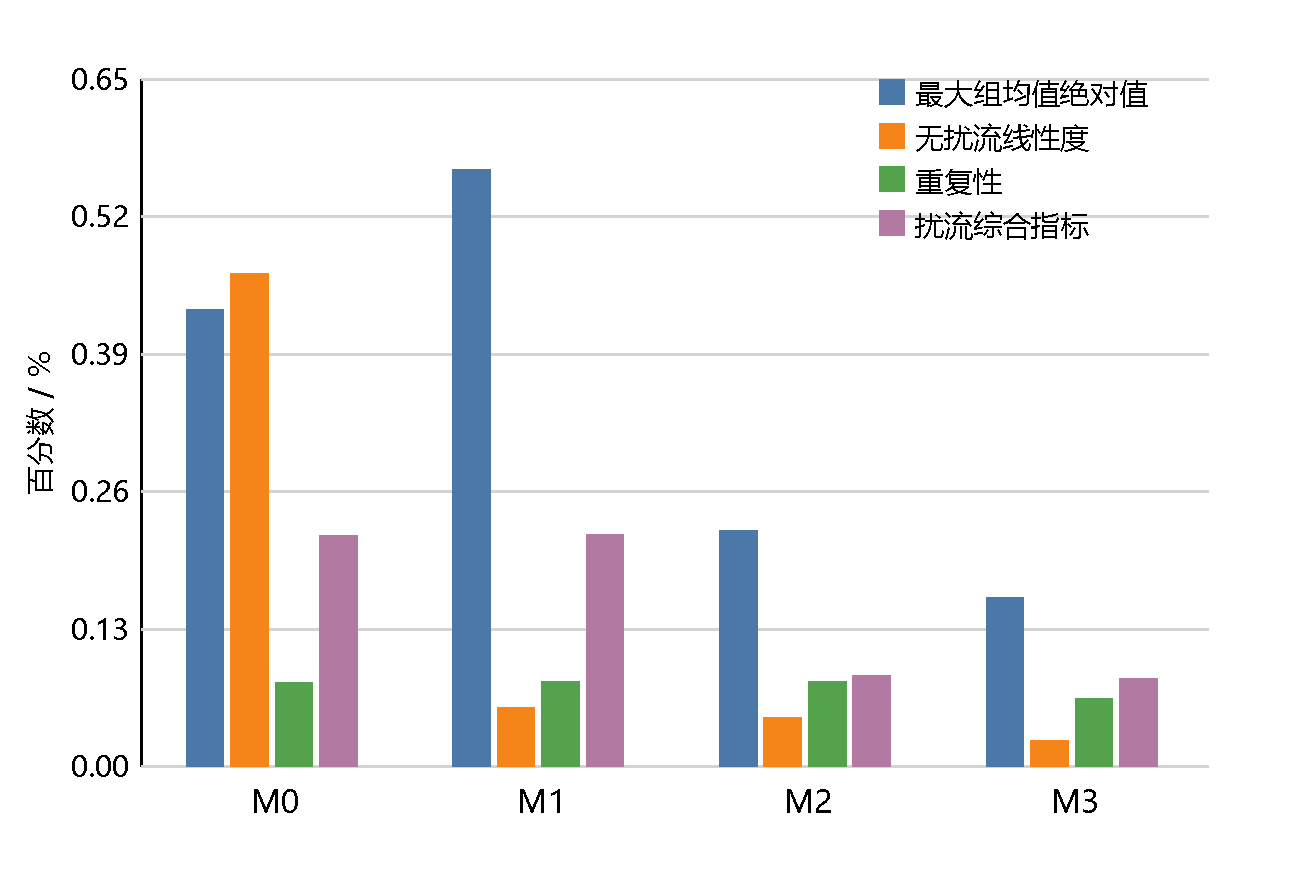
\includegraphics[width=0.70\textwidth]{../figures/fig_krr_ablation_metrics.pdf}
  \caption{四级消融模型与关键指标对比}
  \label{fig:krr_ablation}
\end{figure}

D0 曲线加入后，$u_{\mathrm{nor},L}$ 从 $0.462931\%$ 降至 $0.055310\%$。这表明正常锚点能够修正流量相关偏差，但该曲线并不知道扰流剖面发生了什么，因而 MAE 反而升到 $0.260279\%$，$u_{\mathrm{nor},d}$ 也几乎没有变化。

紧凑特征进入 Ridge 后，MAE 降为 $0.091290\%$，$u_{\mathrm{nor},d}$ 降为 $0.085595\%$。换用 RBF-KRR，MAE 继续下降至 $0.055176\%$，$u_{\mathrm{nor},L}$ 与 $u_{\mathrm{nor},d}$ 均跨过达标线，超限项只剩 $2$ 项。改善来自各层的接续作用，不能只归因于核回归算法本身。

\begin{table}[H]
\centering
\caption{最终主线四级消融结果}
\label{tab:krr_ablation}
\scriptsize
\setlength{\tabcolsep}{3.8pt}
\renewcommand{\arraystretch}{0.92}
\begin{tabular}{lcccccc}
\toprule
阶段 & MAE(\%) & 分组通过 & $u_{\mathrm{nor},L}$(\%) & $u_{\mathrm{nor},r}$(\%) & $u_{\mathrm{nor},d}$(\%) & 超限项 \\
\midrule
Phys6 & 0.179991 & 2/7 & 0.462931 & 0.079400 & 0.217668 & 5 \\
Phys6 + D0 曲线 & 0.260279 & 1/7 & 0.055310 & 0.079728 & 0.218491 & 5 \\
+ Ridge 线性残差 & 0.091290 & 3/7 & 0.046127 & 0.080151 & 0.085595 & 4 \\
+ RBF-KRR & 0.055176 & 3/7 & 0.024645 & 0.064035 & 0.083017 & 2 \\
\bottomrule
\end{tabular}
\end{table}

在主分层标签盲验证中，RBF-KRR 模型取得
\begin{equation}
\mathrm{MAE}=0.055176\%.
\end{equation}
关键达标指标为
\begin{equation}
\max_g|\bar e_g|=0.159304\%\le 0.2\%,
\end{equation}
\begin{equation}
\begin{aligned}
u_{\mathrm{nor},L}&=0.024645\%<0.036\%,\\
u_{\mathrm{nor},r}&=0.064035\%>0.040\%.
\end{aligned}
\end{equation}
\begin{equation}
u_{\mathrm{nor},d}=0.083017\%<0.115\%.
\end{equation}
该模型的平均精度、最大组均值误差、无扰流线性度和扰流综合指标均满足要求，但最大组内重复性超过阈值，评价组通过率为 $3/7$。因此，RBF-KRR 在该划分下具有较好的综合性能，组内重复性是它的主要限制。

\begin{figure}[H]
  \centering
  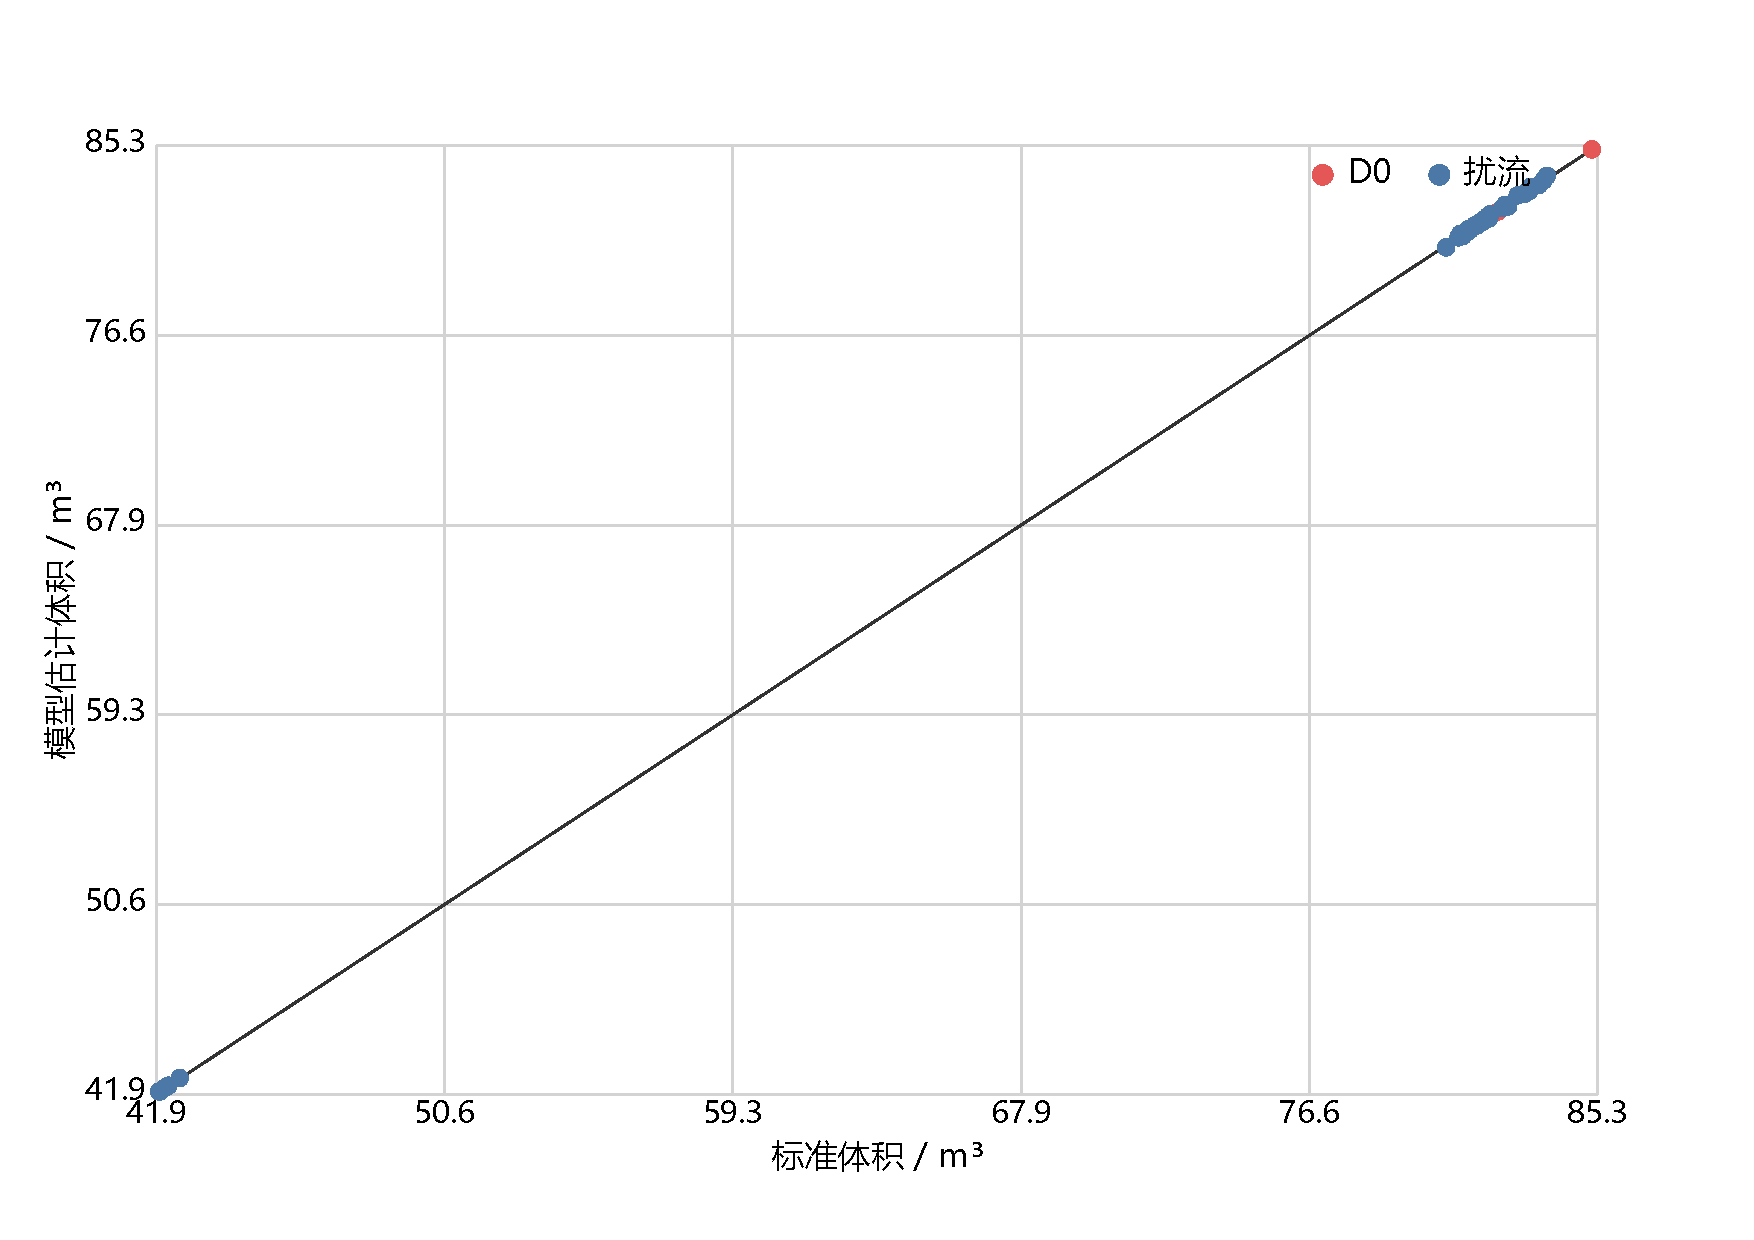
\includegraphics[width=0.70\textwidth]{../figures/fig_prediction_consistency.pdf}
  \caption{RBF-KRR 验证集预测体积与标准体积的一致性}
  \label{fig:prediction_consistency}
\end{figure}

图~\ref{fig:prediction_consistency} 中大部分样本分布在理想一致线附近，说明模型对体积主尺度和系统偏差的控制较好，且未出现明显的整体方向性偏移。然而，散点接近一致线只能反映窗口级预测精度，不能替代同日期、同流量点评价组的重复性检验。$u_{\mathrm{nor},r}=0.064035\%$ 的超限表明，当前紧凑特征仍没有充分解释少数组内的短时状态变化，这也是后续引入逐秒稳定性特征的直接原因。

\subsection{最终推荐模型：双核 KRR 与受约束后校准}

RBF-KRR 的平均误差和扰流漂移已有明显改善，但最坏组重复性仍超过阈值。以附件 6 的逐秒原始声道序列为基础，我们进一步构造物理--稳定性双核 KRR。物理核由紧凑物理特征生成，稳定性核由时差相对离散度、漂移、同步相关、Hampel 异常值替换率、声道波动和 A/B 不匹配等特征生成。两个核按
\begin{equation}
\begin{aligned}
K_{\mathrm{DK}}
&=(1-\beta)K_{\mathrm{physical}}+\beta K_{\mathrm{stab}},\\
K_{\mathrm{physical}}
&=\exp(-\gamma_p d_p^2),\\
K_{\mathrm{stab}}
&=\exp(-\gamma_s d_s^2).
\end{aligned}
\end{equation}
组合，其中 $K_{\mathrm{stab}}$ 表示逐秒稳定性特征核，$\gamma_p=0.05$、$\gamma_s=0.005$、$\beta=0.5$、$\lambda=0.3$。该结构采用 Sch\"olkopf 与 Smola 提出的核正则化思想\cite{Scholkopf2002LearningKernels}。Sakhavi 和 Nouri 的研究表明，多声道速度剖面需要采用独立特征描述\cite{Sakhavi2022GeneralizedProfile}；Li 等的自适应去噪研究说明，窗口内离散度与漂移能够反映观测稳定性\cite{Li2025VMDDenoising}。据此，本文分别构造物理核与稳定性核并进行加权融合。对 $38$ 组候选参数在 $40$ 个按 $h$ 分层的标签盲划分上进行评价，依据超限项数、归一化超限程度、MAE 和分组通过率的中位数确定上述参数。在 $40$ 个划分中，该配置均未实现全部指标同时达标；完整 $159$ 个窗口的样本内 MAE 为 $0.056596\%$，分组通过率为 $13/30$，$u_{\mathrm{nor},L}=0.038713\%$、$u_{\mathrm{nor},r}=0.114864\%$、$u_{\mathrm{nor},d}=0.166680\%$。附件 6 特征增强了窗口稳定性的描述能力，但还不足以控制最坏组重复性。为进一步平衡线性度、重复性和扰流综合指标，本文在双核 KRR 上建立受约束 D0-RBF 后校准层。

最终模型首先按确定的双核参数在完整标定集上重新估计 $\hat V_i^{(\mathrm{DK})}$，随后增加受约束校准层。紧凑特征中的流量尺度记为 $q_i^{(c)}=(\mathrm{flow\ point}_i-50)/30$，D0 线性度曲线采用中心化尺度 $q_i^{(L)}=(\mathrm{flow\ point}_i-70)/30$。最终模型为
\begin{equation}
\begin{aligned}
\hat V_i^{(\mathrm{PC})}
&=\hat V_i^{(\mathrm{DK})}
\left[1+\frac{\Delta_i^{(\mathrm{PC})}}{100}\right],\\
\Delta_i^{(\mathrm{PC})}
&=\mathrm{clip}\left(
\ell(q_i^{(L)})+\rho f_{\mathrm{RBF}}(\boldsymbol z_i),
-0.80,\ 0.80
\right).
\end{aligned}
\label{eq:postcalibrated_dual_kernel_model}
\end{equation}
其中 $\ell(q_i^{(L)})$ 为 D0 正常窗口拟合的线性度校准曲线，$f_{\mathrm{RBF}}$ 为紧凑物理特征与逐秒稳定性特征共同构成的 RBF 校准函数，$\rho$ 为收缩系数。修正幅度限制为 $\pm0.80\%$。固定双核 KRR 结构后，共比较 $5$ 种 D0 曲线、$3$ 组运行时特征、$5$ 个核宽度、$6$ 个正则化系数和 $3$ 个收缩系数，形成 $1350$ 个受约束候选。依据工程阈值通过情况、分组失败数、超限程度、修正幅度和 MAE，确定核宽度 $\gamma=0.1$、正则化系数 $\lambda=0.01$、收缩系数 $\rho=0.75$，并采用线性 D0 校准曲线。

表~\ref{tab:model_evolution_postcalibrated} 汇总各阶段结果。其中，标签盲验证用于评价模型对未参与训练窗口的预测能力，同样本全量标定用于估计给定标定窗口的拟合效果，两种评价口径分别列示。

\begin{table}[H]
\centering
\caption{模型演进与全量标定结果比较}
\label{tab:model_evolution_postcalibrated}
\scriptsize
\setlength{\tabcolsep}{2.5pt}
\begin{tabular}{p{0.20\textwidth}p{0.16\textwidth}cccccc}
\toprule
阶段 & 评价口径 & MAE & 分组 & $\max|\bar e_g|$ & $u_{\mathrm{nor},L}$ & $u_{\mathrm{nor},r}$ & $u_{\mathrm{nor},d}$ \\
\midrule
高维多项式近插值 & 159窗口样本内 & $4.78\!\times\!10^{-9}$ & 30/30 & $7.12\!\times\!10^{-9}$ & $3.86\!\times\!10^{-10}$ & $2.30\!\times\!10^{-8}$ & $2.34\!\times\!10^{-8}$ \\
ANN 对照 & 标签盲验证 & 0.070924 & 3/7 & 0.147747 & 0.066138 & 0.078277 & 0.090823 \\
紧凑 KRR & 标签盲验证 & 0.055176 & 3/7 & 0.159304 & 0.024645 & 0.064035 & 0.083017 \\
物理--稳定性双核 KRR & 159窗口样本内 & 0.056596 & 13/30 & 0.088743 & 0.038713 & 0.114864 & 0.166680 \\
受约束 D0-RBF 后校准双核 KRR & 同样本全量标定 & 0.015891 & 30/30 & 0.028735 & 0.009585 & 0.033630 & 0.048435 \\
\bottomrule
\end{tabular}
\par\smallskip
{\footnotesize 注：除“分组”外，其余指标单位均为 \%。}
\end{table}

由表~\ref{tab:model_evolution_postcalibrated} 可知，高维多项式模型的样本内误差最低，但留一日期误差明显增大；ANN 能够刻画非线性残差，但在小样本条件下稳定性不足；紧凑 RBF-KRR 和物理--稳定性双核 KRR 提高了模型的物理可解释性与窗口稳定性描述能力，最坏组重复性仍是主要限制。受约束 D0-RBF 后校准双核 KRR 在全量标定数据上进一步平衡线性度、重复性和扰流漂移，用于生成最终体积估计。其数值反映给定标定窗口的拟合效果，未知日期和扰流状态仍需通过独立数据检验。

问题三的聚类结果显示，D1--D8 在在线特征空间中没有形成稳定的多类边界；$K=2$ 时主要将 D3 单独分出，其余扰流状态仍大量重叠。硬聚类专家会把前级错分继续传递到体积估计，因此本文采用统一 RBF-KRR 对局部相似剖面连续加权。最终体积估计使用受约束 D0-RBF 后校准双核 KRR，适用于题目给定的标定窗口；新增日期或未知扰流状态需由独立样本重新评价。

\subsection{结果分析}

模型演进表明，误差均值下降并不等于工程指标同步改善。紧凑 RBF-KRR 在标签盲验证中的 MAE 为 $0.055176\%$，无扰流线性度和扰流综合指标分别为 $0.024645\%$ 与 $0.083017\%$，均已满足阈值；但重复性为 $0.064035\%$，评价组仅通过 $3/7$，说明少数组内短时变化仍未被充分描述。

加入逐秒稳定性信息后，双核结构能够把剖面差异与窗口波动分开度量，但在完整标定样本内仍只有 $13/30$ 个评价组通过。进一步采用受约束无扰流后校准后，题目给定 $159$ 个标定窗口上的 MAE 降为 $0.015891\%$，分组通过率为 $30/30$，三项综合指标分别为 $0.009585\%$、$0.033630\%$ 和 $0.048435\%$。

上述结果对应两种不同证据。标签盲划分反映模型对未参与训练窗口的预测能力，而后校准双核 KRR 的全部达标结果属于同样本全量标定，只能说明其适合生成题目给定窗口的最终体积估计。对新增日期或未知扰流状态，仍需固定特征、核参数和校准形式后使用独立数据复验。
